\documentclass[twoside]{book}

% Packages required by doxygen
\usepackage{fixltx2e}
\usepackage{calc}
\usepackage{doxygen}
\usepackage[export]{adjustbox} % also loads graphicx
\usepackage{graphicx}
\usepackage[utf8]{inputenc}
\usepackage{makeidx}
\usepackage{multicol}
\usepackage{multirow}
\PassOptionsToPackage{warn}{textcomp}
\usepackage{textcomp}
\usepackage[nointegrals]{wasysym}
\usepackage[table]{xcolor}

% Font selection
\usepackage[T1]{fontenc}
\usepackage[scaled=.90]{helvet}
\usepackage{courier}
\usepackage{amssymb}
\usepackage{sectsty}
\renewcommand{\familydefault}{\sfdefault}
\allsectionsfont{%
  \fontseries{bc}\selectfont%
  \color{darkgray}%
}
\renewcommand{\DoxyLabelFont}{%
  \fontseries{bc}\selectfont%
  \color{darkgray}%
}
\newcommand{\+}{\discretionary{\mbox{\scriptsize$\hookleftarrow$}}{}{}}

% Page & text layout
\usepackage{geometry}
\geometry{%
  a4paper,%
  top=2.5cm,%
  bottom=2.5cm,%
  left=2.5cm,%
  right=2.5cm%
}
\tolerance=750
\hfuzz=15pt
\hbadness=750
\setlength{\emergencystretch}{15pt}
\setlength{\parindent}{0cm}
\setlength{\parskip}{0.2cm}
\makeatletter
\renewcommand{\paragraph}{%
  \@startsection{paragraph}{4}{0ex}{-1.0ex}{1.0ex}{%
    \normalfont\normalsize\bfseries\SS@parafont%
  }%
}
\renewcommand{\subparagraph}{%
  \@startsection{subparagraph}{5}{0ex}{-1.0ex}{1.0ex}{%
    \normalfont\normalsize\bfseries\SS@subparafont%
  }%
}
\makeatother

% Headers & footers
\usepackage{fancyhdr}
\pagestyle{fancyplain}
\fancyhead[LE]{\fancyplain{}{\bfseries\thepage}}
\fancyhead[CE]{\fancyplain{}{}}
\fancyhead[RE]{\fancyplain{}{\bfseries\leftmark}}
\fancyhead[LO]{\fancyplain{}{\bfseries\rightmark}}
\fancyhead[CO]{\fancyplain{}{}}
\fancyhead[RO]{\fancyplain{}{\bfseries\thepage}}
\fancyfoot[LE]{\fancyplain{}{}}
\fancyfoot[CE]{\fancyplain{}{}}
\fancyfoot[RE]{\fancyplain{}{\bfseries\scriptsize Generated on Thu Oct 22 2015 13\+:29\+:25 for Serbus by Doxygen }}
\fancyfoot[LO]{\fancyplain{}{\bfseries\scriptsize Generated on Thu Oct 22 2015 13\+:29\+:25 for Serbus by Doxygen }}
\fancyfoot[CO]{\fancyplain{}{}}
\fancyfoot[RO]{\fancyplain{}{}}
\renewcommand{\footrulewidth}{0.4pt}
\renewcommand{\chaptermark}[1]{%
  \markboth{#1}{}%
}
\renewcommand{\sectionmark}[1]{%
  \markright{\thesection\ #1}%
}

% Indices & bibliography
\usepackage{natbib}
\usepackage[titles]{tocloft}
\setcounter{tocdepth}{3}
\setcounter{secnumdepth}{5}
\makeindex

% Hyperlinks (required, but should be loaded last)
\usepackage{ifpdf}
\ifpdf
  \usepackage[pdftex,pagebackref=true]{hyperref}
\else
  \usepackage[ps2pdf,pagebackref=true]{hyperref}
\fi
\hypersetup{%
  colorlinks=true,%
  linkcolor=blue,%
  citecolor=blue,%
  unicode%
}

% Custom commands
\newcommand{\clearemptydoublepage}{%
  \newpage{\pagestyle{empty}\cleardoublepage}%
}


%===== C O N T E N T S =====

\begin{document}

% Titlepage & ToC
\hypersetup{pageanchor=false,
             bookmarks=true,
             bookmarksnumbered=true,
             pdfencoding=unicode
            }
\pagenumbering{roman}
\begin{titlepage}
\vspace*{7cm}
\begin{center}%
{\Large Serbus \\[1ex]\large v1.\+0.\+2 }\\
\vspace*{1cm}
{\large Generated by Doxygen 1.8.9.1}\\
\vspace*{0.5cm}
{\small Thu Oct 22 2015 13:29:25}\\
\end{center}
\end{titlepage}
\clearemptydoublepage
\tableofcontents
\clearemptydoublepage
\pagenumbering{arabic}
\hypersetup{pageanchor=true}

%--- Begin generated contents ---
\chapter{Main Page}
\label{index}\hypertarget{index}{}Copyright (c) 2015 -\/ Gray Cat Labs -\/ \href{https://graycat.io}{\tt https\+://graycat.\+io}

\href{https://github.com/graycatlabs/serbus}{\tt https\+://github.\+com/graycatlabs/serbus}

Serbus provides basic C A\+P\+Is for the I2\+C and S\+P\+I serial bus protocols on G\+N\+U/\+Linux based systems, as well as a Python package built on top of them.

It\textquotesingle{}s really just a wrapper for the ioctl commands provided by the standard Linux I2\+C and S\+P\+I drivers, so it should be pretty universal. That said, I\textquotesingle{}ve currently only tested it extensively on the Beagle\+Bone Black, so use it at your own risk! (And let me know if it\textquotesingle{}s working for you on another system)

\subsection*{Contributing}

Have something to contribute? Great! This project follows the Contributor Covenant Code of Conduct, so be sure to read {\ttfamily \hyperlink{code__of__conduct_8md_source}{code\+\_\+of\+\_\+conduct.\+md}}.

\subsection*{License}

Released under the M\+I\+T license. \begin{DoxyVerb}Permission is hereby granted, free of charge, to any person obtaining a copy
of this software and associated documentation files (the "Software"), to deal
in the Software without restriction, including without limitation the rights
to use, copy, modify, merge, publish, distribute, sublicense, and/or sell
copies of the Software, and to permit persons to whom the Software is
furnished to do so, subject to the following conditions:

The above copyright notice and this permission notice shall be included in
all copies or substantial portions of the Software.

THE SOFTWARE IS PROVIDED "AS IS", WITHOUT WARRANTY OF ANY KIND, EXPRESS OR
IMPLIED, INCLUDING BUT NOT LIMITED TO THE WARRANTIES OF MERCHANTABILITY,
FITNESS FOR A PARTICULAR PURPOSE AND NONINFRINGEMENT. IN NO EVENT SHALL THE
AUTHORS OR COPYRIGHT HOLDERS BE LIABLE FOR ANY CLAIM, DAMAGES OR OTHER
LIABILITY, WHETHER IN AN ACTION OF CONTRACT, TORT OR OTHERWISE, ARISING FROM,
OUT OF OR IN CONNECTION WITH THE SOFTWARE OR THE USE OR OTHER DEALINGS IN
THE SOFTWARE. \end{DoxyVerb}
 
\chapter{Contributor Code of Conduct}
\label{md_code_of_conduct}
\hypertarget{md_code_of_conduct}{}
As contributors and maintainers of this project, and in the interest of fostering an open and welcoming community, we pledge to respect all people who contribute through reporting issues, posting feature requests, updating documentation, submitting pull requests or patches, and other activities.

We are committed to making participation in this project a harassment-\/free experience for everyone, regardless of level of experience, gender, gender identity and expression, sexual orientation, disability, personal appearance, body size, race, ethnicity, age, religion, or nationality.

Examples of unacceptable behavior by participants include\+:


\begin{DoxyItemize}
\item The use of sexualized language or imagery
\item Personal attacks
\item Trolling or insulting/derogatory comments
\item Public or private harassment
\item Publishing other\textquotesingle{}s private information, such as physical or electronic addresses, without explicit permission
\item Other unethical or unprofessional conduct.
\end{DoxyItemize}

Project maintainers have the right and responsibility to remove, edit, or reject comments, commits, code, wiki edits, issues, and other contributions that are not aligned to this Code of Conduct. By adopting this Code of Conduct, project maintainers commit themselves to fairly and consistently applying these principles to every aspect of managing this project. Project maintainers who do not follow or enforce the Code of Conduct may be permanently removed from the project team.

This code of conduct applies both within project spaces and in public spaces when an individual is representing the project or its community.

Instances of abusive, harassing, or otherwise unacceptable behavior may be reported by opening an issue or contacting one or more of the project maintainers.

This Code of Conduct is adapted from the \href{http://contributor-covenant.org}{\tt Contributor Covenant}, version 1.\+2.\+0, available at \href{http://contributor-covenant.org/version/1/2/0/}{\tt http\+://contributor-\/covenant.\+org/version/1/2/0/} 
\chapter{File Index}
\section{File List}
Here is a list of all documented files with brief descriptions\+:\begin{DoxyCompactList}
\item\contentsline{section}{include/\hyperlink{i2cdriver_8h}{i2cdriver.\+h} \\*A basic driver for controlling Linux I2\+C interfaces }{\pageref{i2cdriver_8h}}{}
\item\contentsline{section}{include/\hyperlink{spidriver_8h}{spidriver.\+h} \\*A basic driver for controlling Linux spidev interfaces }{\pageref{spidriver_8h}}{}
\end{DoxyCompactList}

\chapter{File Documentation}
\hypertarget{i2cdriver_8h}{}\section{include/i2cdriver.h File Reference}
\label{i2cdriver_8h}\index{include/i2cdriver.\+h@{include/i2cdriver.\+h}}


A basic driver for controlling Linux I2\+C interfaces.  


{\ttfamily \#include $<$stdint.\+h$>$}\\*
Include dependency graph for i2cdriver.\+h\+:\nopagebreak
\begin{figure}[H]
\begin{center}
\leavevmode
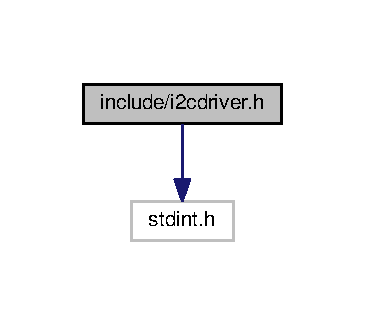
\includegraphics[width=175pt]{i2cdriver_8h__incl}
\end{center}
\end{figure}
\subsection*{Functions}
\begin{DoxyCompactItemize}
\item 
int \hyperlink{i2cdriver_8h_a5df2435ff8cec2b6de06a473cf427864}{I2\+C\+\_\+open} (uint8\+\_\+t bus)
\begin{DoxyCompactList}\small\item\em Opens the /dev/i2c-\/\mbox{[}bus\mbox{]} interface. \end{DoxyCompactList}\item 
void \hyperlink{i2cdriver_8h_a097ccdcc5540327f0df6118700a68364}{I2\+C\+\_\+close} (int i2c\+\_\+fd)
\begin{DoxyCompactList}\small\item\em Closes the given I2\+C interface. \end{DoxyCompactList}\item 
int \hyperlink{i2cdriver_8h_abc7c776c69df4882cb483e30eb4404d0}{I2\+C\+\_\+enable10\+Bit\+Addressing} (int i2c\+\_\+fd)
\begin{DoxyCompactList}\small\item\em Enables 10-\/bit addressing the given I2\+C interface. \end{DoxyCompactList}\item 
int \hyperlink{i2cdriver_8h_a1d2c05b3127b4520cc09ee3b80709a8c}{I2\+C\+\_\+disable10\+Bit\+Addressing} (int i2c\+\_\+fd)
\begin{DoxyCompactList}\small\item\em Disables 10-\/bit addressing the given I2\+C interface. \end{DoxyCompactList}\item 
int \hyperlink{i2cdriver_8h_aa78b1a1354344e7010843cffe962df89}{I2\+C\+\_\+set\+Slave\+Address} (int i2c\+\_\+fd, int addr)
\begin{DoxyCompactList}\small\item\em Sets the I2\+C slave address to communicate with. \end{DoxyCompactList}\item 
int \hyperlink{i2cdriver_8h_ac9c2d06e7ea0e9c01a840841743b27c5}{I2\+C\+\_\+read} (int i2c\+\_\+fd, void $\ast$rx\+\_\+buffer, int n\+\_\+bytes)
\begin{DoxyCompactList}\small\item\em Reads a block from the given I2\+C interface. \end{DoxyCompactList}\item 
int \hyperlink{i2cdriver_8h_a4fb00c476124be12a5484290051cc465}{I2\+C\+\_\+read\+Transaction} (int i2c\+\_\+fd, uint8\+\_\+t byte, void $\ast$rx\+\_\+buffer, int n\+\_\+bytes)
\begin{DoxyCompactList}\small\item\em Writes the given command then reads a block from the given I2\+C interface. \end{DoxyCompactList}\item 
int \hyperlink{i2cdriver_8h_a4889f4597892b63190e1d9e4dd4bb209}{I2\+C\+\_\+write} (int i2c\+\_\+fd, void $\ast$tx\+\_\+buffer, int n\+\_\+bytes)
\begin{DoxyCompactList}\small\item\em Writes a block to the given I2\+C interface. \end{DoxyCompactList}\end{DoxyCompactItemize}


\subsection{Detailed Description}
A basic driver for controlling Linux I2\+C interfaces. 

\begin{DoxyAuthor}{Author}
Alex Hiam -\/ \href{mailto:alex@graycat.io}{\tt alex@graycat.\+io}
\end{DoxyAuthor}
Requires an I2\+C Kernel driver be loaded to expose /dev/i2c-\/\+N interfaces which provide the standard Linux I2\+C ioctls. This driver is really just an ioctl wrapper. 

\subsection{Function Documentation}
\hypertarget{i2cdriver_8h_a097ccdcc5540327f0df6118700a68364}{}\index{i2cdriver.\+h@{i2cdriver.\+h}!I2\+C\+\_\+close@{I2\+C\+\_\+close}}
\index{I2\+C\+\_\+close@{I2\+C\+\_\+close}!i2cdriver.\+h@{i2cdriver.\+h}}
\subsubsection[{I2\+C\+\_\+close}]{\setlength{\rightskip}{0pt plus 5cm}void I2\+C\+\_\+close (
\begin{DoxyParamCaption}
\item[{int}]{i2c\+\_\+fd}
\end{DoxyParamCaption}
)}\label{i2cdriver_8h_a097ccdcc5540327f0df6118700a68364}


Closes the given I2\+C interface. 


\begin{DoxyParams}{Parameters}
{\em i2c\+\_\+fd} & I2\+C bus file descriptor to close \\
\hline
\end{DoxyParams}
\hypertarget{i2cdriver_8h_a1d2c05b3127b4520cc09ee3b80709a8c}{}\index{i2cdriver.\+h@{i2cdriver.\+h}!I2\+C\+\_\+disable10\+Bit\+Addressing@{I2\+C\+\_\+disable10\+Bit\+Addressing}}
\index{I2\+C\+\_\+disable10\+Bit\+Addressing@{I2\+C\+\_\+disable10\+Bit\+Addressing}!i2cdriver.\+h@{i2cdriver.\+h}}
\subsubsection[{I2\+C\+\_\+disable10\+Bit\+Addressing}]{\setlength{\rightskip}{0pt plus 5cm}int I2\+C\+\_\+disable10\+Bit\+Addressing (
\begin{DoxyParamCaption}
\item[{int}]{i2c\+\_\+fd}
\end{DoxyParamCaption}
)}\label{i2cdriver_8h_a1d2c05b3127b4520cc09ee3b80709a8c}


Disables 10-\/bit addressing the given I2\+C interface. 


\begin{DoxyParams}{Parameters}
{\em i2c\+\_\+fd} & I2\+C file descriptor\\
\hline
\end{DoxyParams}
\begin{DoxyReturn}{Returns}
Returns 0 if successful, ioctl error code otherwise 
\end{DoxyReturn}
\hypertarget{i2cdriver_8h_abc7c776c69df4882cb483e30eb4404d0}{}\index{i2cdriver.\+h@{i2cdriver.\+h}!I2\+C\+\_\+enable10\+Bit\+Addressing@{I2\+C\+\_\+enable10\+Bit\+Addressing}}
\index{I2\+C\+\_\+enable10\+Bit\+Addressing@{I2\+C\+\_\+enable10\+Bit\+Addressing}!i2cdriver.\+h@{i2cdriver.\+h}}
\subsubsection[{I2\+C\+\_\+enable10\+Bit\+Addressing}]{\setlength{\rightskip}{0pt plus 5cm}int I2\+C\+\_\+enable10\+Bit\+Addressing (
\begin{DoxyParamCaption}
\item[{int}]{i2c\+\_\+fd}
\end{DoxyParamCaption}
)}\label{i2cdriver_8h_abc7c776c69df4882cb483e30eb4404d0}


Enables 10-\/bit addressing the given I2\+C interface. 


\begin{DoxyParams}{Parameters}
{\em i2c\+\_\+fd} & I2\+C file descriptor\\
\hline
\end{DoxyParams}
\begin{DoxyReturn}{Returns}
Returns 0 if successful, ioctl error code otherwise 
\end{DoxyReturn}
\hypertarget{i2cdriver_8h_a5df2435ff8cec2b6de06a473cf427864}{}\index{i2cdriver.\+h@{i2cdriver.\+h}!I2\+C\+\_\+open@{I2\+C\+\_\+open}}
\index{I2\+C\+\_\+open@{I2\+C\+\_\+open}!i2cdriver.\+h@{i2cdriver.\+h}}
\subsubsection[{I2\+C\+\_\+open}]{\setlength{\rightskip}{0pt plus 5cm}int I2\+C\+\_\+open (
\begin{DoxyParamCaption}
\item[{uint8\+\_\+t}]{bus}
\end{DoxyParamCaption}
)}\label{i2cdriver_8h_a5df2435ff8cec2b6de06a473cf427864}


Opens the /dev/i2c-\/\mbox{[}bus\mbox{]} interface. 


\begin{DoxyParams}{Parameters}
{\em bus} & I2\+C bus number\\
\hline
\end{DoxyParams}
\begin{DoxyReturn}{Returns}
Returns the file descriptor for the I2\+C bus. 
\end{DoxyReturn}
\hypertarget{i2cdriver_8h_ac9c2d06e7ea0e9c01a840841743b27c5}{}\index{i2cdriver.\+h@{i2cdriver.\+h}!I2\+C\+\_\+read@{I2\+C\+\_\+read}}
\index{I2\+C\+\_\+read@{I2\+C\+\_\+read}!i2cdriver.\+h@{i2cdriver.\+h}}
\subsubsection[{I2\+C\+\_\+read}]{\setlength{\rightskip}{0pt plus 5cm}int I2\+C\+\_\+read (
\begin{DoxyParamCaption}
\item[{int}]{i2c\+\_\+fd, }
\item[{void $\ast$}]{rx\+\_\+buffer, }
\item[{int}]{n\+\_\+bytes}
\end{DoxyParamCaption}
)}\label{i2cdriver_8h_ac9c2d06e7ea0e9c01a840841743b27c5}


Reads a block from the given I2\+C interface. 

Reads {\ttfamily n\+\_\+bytes} from the current slave address on the given I2\+C interface. and puts them into the given buffer.


\begin{DoxyParams}{Parameters}
{\em i2c\+\_\+fd} & I2\+C file descriptor \\
\hline
{\em rx\+\_\+buffer} & pointer to an array, already initialized to the required size \\
\hline
{\em n\+\_\+bytes} & the number of bytes to read into rx\+\_\+buffer\\
\hline
\end{DoxyParams}
\begin{DoxyReturn}{Returns}
Returns 0 if successful, file access error code otherwise 
\end{DoxyReturn}
\hypertarget{i2cdriver_8h_a4fb00c476124be12a5484290051cc465}{}\index{i2cdriver.\+h@{i2cdriver.\+h}!I2\+C\+\_\+read\+Transaction@{I2\+C\+\_\+read\+Transaction}}
\index{I2\+C\+\_\+read\+Transaction@{I2\+C\+\_\+read\+Transaction}!i2cdriver.\+h@{i2cdriver.\+h}}
\subsubsection[{I2\+C\+\_\+read\+Transaction}]{\setlength{\rightskip}{0pt plus 5cm}int I2\+C\+\_\+read\+Transaction (
\begin{DoxyParamCaption}
\item[{int}]{i2c\+\_\+fd, }
\item[{uint8\+\_\+t}]{byte, }
\item[{void $\ast$}]{rx\+\_\+buffer, }
\item[{int}]{n\+\_\+bytes}
\end{DoxyParamCaption}
)}\label{i2cdriver_8h_a4fb00c476124be12a5484290051cc465}


Writes the given command then reads a block from the given I2\+C interface. 

Writes the given byte, then immediately reads n\+\_\+bytes bytes from the current slave address on the given I2\+C interface. Useful for things like reading register values from memory mapped devices.


\begin{DoxyParams}{Parameters}
{\em i2c\+\_\+fd} & I2\+C file descriptor \\
\hline
{\em byte} & the byte to write before reading \\
\hline
{\em rx\+\_\+buffer} & pointer to an array, already initialized to the required size \\
\hline
{\em n\+\_\+bytes} & the number of bytes to read into rx\+\_\+buffer\\
\hline
\end{DoxyParams}
\begin{DoxyReturn}{Returns}
Returns 0 if successful, file access error code otherwise 
\end{DoxyReturn}
\hypertarget{i2cdriver_8h_aa78b1a1354344e7010843cffe962df89}{}\index{i2cdriver.\+h@{i2cdriver.\+h}!I2\+C\+\_\+set\+Slave\+Address@{I2\+C\+\_\+set\+Slave\+Address}}
\index{I2\+C\+\_\+set\+Slave\+Address@{I2\+C\+\_\+set\+Slave\+Address}!i2cdriver.\+h@{i2cdriver.\+h}}
\subsubsection[{I2\+C\+\_\+set\+Slave\+Address}]{\setlength{\rightskip}{0pt plus 5cm}int I2\+C\+\_\+set\+Slave\+Address (
\begin{DoxyParamCaption}
\item[{int}]{i2c\+\_\+fd, }
\item[{int}]{addr}
\end{DoxyParamCaption}
)}\label{i2cdriver_8h_aa78b1a1354344e7010843cffe962df89}


Sets the I2\+C slave address to communicate with. 

Sets the I2\+C slave address that\textquotesingle{}s sent with all subsequent I2\+C transactions on the given I2\+C bus, until I2\+C\+\_\+set\+Slave\+Address is called again with a new address.


\begin{DoxyParams}{Parameters}
{\em i2c\+\_\+fd} & I2\+C file descriptor \\
\hline
{\em addr} & the 7-\/ or 10-\/bit address of the slave device\\
\hline
\end{DoxyParams}
\begin{DoxyReturn}{Returns}
Returns 0 if successful, ioctl error code otherwise 
\end{DoxyReturn}
\hypertarget{i2cdriver_8h_a4889f4597892b63190e1d9e4dd4bb209}{}\index{i2cdriver.\+h@{i2cdriver.\+h}!I2\+C\+\_\+write@{I2\+C\+\_\+write}}
\index{I2\+C\+\_\+write@{I2\+C\+\_\+write}!i2cdriver.\+h@{i2cdriver.\+h}}
\subsubsection[{I2\+C\+\_\+write}]{\setlength{\rightskip}{0pt plus 5cm}int I2\+C\+\_\+write (
\begin{DoxyParamCaption}
\item[{int}]{i2c\+\_\+fd, }
\item[{void $\ast$}]{tx\+\_\+buffer, }
\item[{int}]{n\+\_\+bytes}
\end{DoxyParamCaption}
)}\label{i2cdriver_8h_a4889f4597892b63190e1d9e4dd4bb209}


Writes a block to the given I2\+C interface. 

Writes n\+\_\+bytes bytes from the given buffer to the current slave address on the given I2\+C interface.


\begin{DoxyParams}{Parameters}
{\em i2c\+\_\+fd} & I2\+C file descriptor \\
\hline
{\em tx\+\_\+buffer} & pointer to an array containing the words to be transmitted \\
\hline
{\em n\+\_\+bytes} & the number of bytes to write from tx\+\_\+buffer\\
\hline
\end{DoxyParams}
\begin{DoxyReturn}{Returns}
Returns 0 if successful, file access error code otherwise 
\end{DoxyReturn}

\hypertarget{spidriver_8h}{}\section{include/spidriver.h File Reference}
\label{spidriver_8h}\index{include/spidriver.\+h@{include/spidriver.\+h}}


A basic driver for controlling Linux spidev interfaces.  


{\ttfamily \#include $<$stdint.\+h$>$}\\*
{\ttfamily \#include $<$linux/spi/spidev.\+h$>$}\\*
Include dependency graph for spidriver.\+h\+:\nopagebreak
\begin{figure}[H]
\begin{center}
\leavevmode
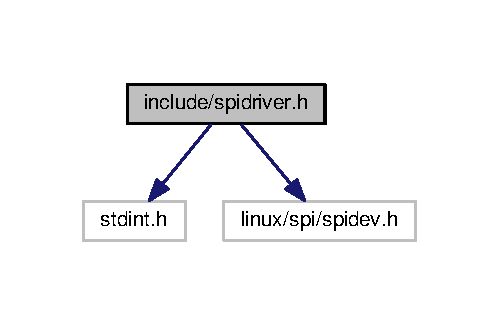
\includegraphics[width=240pt]{spidriver_8h__incl}
\end{center}
\end{figure}
\subsection*{Enumerations}
\begin{DoxyCompactItemize}
\item 
enum \hyperlink{spidriver_8h_a31bd35a1aecbf364e888c14b090ff3d4}{S\+P\+I\+\_\+bit\+\_\+order} \{ \hyperlink{spidriver_8h_a31bd35a1aecbf364e888c14b090ff3d4a3fa35f661bf7fbb96c05ff70827553be}{S\+P\+I\+\_\+\+M\+S\+B\+F\+I\+R\+S\+T}, 
\hyperlink{spidriver_8h_a31bd35a1aecbf364e888c14b090ff3d4a183d076e845f5ea5d99465cd6aff505f}{S\+P\+I\+\_\+\+L\+S\+B\+F\+I\+R\+S\+T}
 \}
\end{DoxyCompactItemize}
\subsection*{Functions}
\begin{DoxyCompactItemize}
\item 
int \hyperlink{spidriver_8h_af608773d4a769343f1967258b273971b}{S\+P\+I\+\_\+open} (uint8\+\_\+t bus, uint8\+\_\+t cs)
\begin{DoxyCompactList}\small\item\em Opens the /dev/spidev\mbox{[}bus\mbox{]}.\mbox{[}cs\mbox{]} interface. \end{DoxyCompactList}\item 
void \hyperlink{spidriver_8h_a7ff9166531a3a53a0204f4814af37984}{S\+P\+I\+\_\+close} (int spidev\+\_\+fd)
\begin{DoxyCompactList}\small\item\em Closes the given spidev interface. \end{DoxyCompactList}\item 
int \hyperlink{spidriver_8h_aecb40c484f3e3aeec9e496e26b75cd7f}{S\+P\+I\+\_\+read} (int spidev\+\_\+fd, void $\ast$rx\+\_\+buffer, int n\+\_\+words)
\begin{DoxyCompactList}\small\item\em Reads from the given spidev interface. \end{DoxyCompactList}\item 
int \hyperlink{spidriver_8h_a665527500ba4a01476e2a0b5cda44d41}{S\+P\+I\+\_\+write} (int spidev\+\_\+fd, void $\ast$tx\+\_\+buffer, int n\+\_\+words)
\begin{DoxyCompactList}\small\item\em Writes to the given spidev interface. \end{DoxyCompactList}\item 
int \hyperlink{spidriver_8h_a597d2232d2925b4e436a7c23eae4d3d3}{S\+P\+I\+\_\+transfer} (int spidev\+\_\+fd, void $\ast$tx\+\_\+buffer, void $\ast$rx\+\_\+buffer, int n\+\_\+words)
\begin{DoxyCompactList}\small\item\em Writes to and reads from the given spidev interface simultaneously. \end{DoxyCompactList}\item 
int \hyperlink{spidriver_8h_ab2adb8ed5190c8c0cc112fceea89098d}{S\+P\+I\+\_\+set\+Bit\+Order} (int spidev\+\_\+fd, \hyperlink{spidriver_8h_a31bd35a1aecbf364e888c14b090ff3d4}{S\+P\+I\+\_\+bit\+\_\+order} bit\+\_\+order)
\begin{DoxyCompactList}\small\item\em Sets the bit order of the given spidev interface. \end{DoxyCompactList}\item 
int \hyperlink{spidriver_8h_ad65e7362ab689c4de7d31f9ab19777fe}{S\+P\+I\+\_\+set\+Bits\+Per\+Word} (int spidev\+\_\+fd, uint8\+\_\+t bits\+\_\+per\+\_\+word)
\begin{DoxyCompactList}\small\item\em Sets the number of bits per word for the given spidev interface. \end{DoxyCompactList}\item 
int \hyperlink{spidriver_8h_ac60f1a39c48d5c3ae9bbed420cce8551}{S\+P\+I\+\_\+get\+Bits\+Per\+Word} (int spidev\+\_\+fd)
\begin{DoxyCompactList}\small\item\em Gets the number of bits per word for the given spidev interface. \end{DoxyCompactList}\item 
int \hyperlink{spidriver_8h_af60601f12d58cb00180f16c245191dda}{S\+P\+I\+\_\+set\+Max\+Frequency} (int spidev\+\_\+fd, uint32\+\_\+t frequency)
\begin{DoxyCompactList}\small\item\em Sets the maximum clock frequency for the given spidev interface. \end{DoxyCompactList}\item 
int \hyperlink{spidriver_8h_a33876b63ecaab993dbdca380bdaa2dab}{S\+P\+I\+\_\+get\+Max\+Frequency} (int spidev\+\_\+fd)
\begin{DoxyCompactList}\small\item\em Gets the maximum clock frequency for the given spidev interface. \end{DoxyCompactList}\item 
int \hyperlink{spidriver_8h_ad02fbb762c5783f45db896b133cdf9ff}{S\+P\+I\+\_\+set\+Clock\+Mode} (int spidev\+\_\+fd, uint8\+\_\+t clock\+\_\+mode)
\begin{DoxyCompactList}\small\item\em Sets the clock mode for the given spidev interface. \end{DoxyCompactList}\item 
int \hyperlink{spidriver_8h_acf0c4b6dd9a5f1bf164d336858ef9d63}{S\+P\+I\+\_\+get\+Clock\+Mode} (int spidev\+\_\+fd)
\begin{DoxyCompactList}\small\item\em Gets the clock mode for the given spidev interface. \end{DoxyCompactList}\item 
int \hyperlink{spidriver_8h_ab7d5d25b529b1c937649a8ef5bb45218}{S\+P\+I\+\_\+set\+C\+S\+Active\+Low} (int spidev\+\_\+fd)
\begin{DoxyCompactList}\small\item\em Sets the given spidev interface\textquotesingle{}s cs signal to be active low. \end{DoxyCompactList}\item 
int \hyperlink{spidriver_8h_a0cb07d57c9422bacb7229e00546ad426}{S\+P\+I\+\_\+set\+C\+S\+Active\+High} (int spidev\+\_\+fd)
\begin{DoxyCompactList}\small\item\em Sets the given spidev interface\textquotesingle{}s cs signal to be active high. \end{DoxyCompactList}\item 
int \hyperlink{spidriver_8h_ab8bffff4f109622f5425c353fd8b5851}{S\+P\+I\+\_\+enable\+C\+S} (int spidev\+\_\+fd)
\begin{DoxyCompactList}\small\item\em Enables the given spidev interface\textquotesingle{}s cs output. \end{DoxyCompactList}\item 
int \hyperlink{spidriver_8h_a765c913618ea80e9ad453d8ab2120b60}{S\+P\+I\+\_\+disable\+C\+S} (int spidev\+\_\+fd)
\begin{DoxyCompactList}\small\item\em Disables the given spidev interface\textquotesingle{}s cs output. \end{DoxyCompactList}\item 
int \hyperlink{spidriver_8h_ad8f59619ae9d1f2d97b0e0969bb612e1}{S\+P\+I\+\_\+enable\+Loopback} (int spidev\+\_\+fd)
\begin{DoxyCompactList}\small\item\em Puts the given spidev interface in loopback mode. \end{DoxyCompactList}\item 
int \hyperlink{spidriver_8h_a0208c430a384927f4a8f0eaf90fe9d41}{S\+P\+I\+\_\+disable\+Loopback} (int spidev\+\_\+fd)
\begin{DoxyCompactList}\small\item\em Disables loopback mode for the given spidev interface. \end{DoxyCompactList}\item 
int \hyperlink{spidriver_8h_af319540760d84fa649545616be122399}{S\+P\+I\+\_\+enable3\+Wire} (int spidev\+\_\+fd)
\begin{DoxyCompactList}\small\item\em Enables 3-\/wire S\+P\+I mode for the given spidev interface. \end{DoxyCompactList}\item 
int \hyperlink{spidriver_8h_a271b02468019ecb7746ea404772b2e6c}{S\+P\+I\+\_\+disable3\+Wire} (int spidev\+\_\+fd)
\begin{DoxyCompactList}\small\item\em Enables 4-\/wire S\+P\+I mode for the given spidev interface. \end{DoxyCompactList}\item 
int \hyperlink{spidriver_8h_a74608d149677e6ac4918457dd426ab51}{S\+P\+I\+\_\+set\+Mode} (int spidev\+\_\+fd, uint8\+\_\+t mode)
\begin{DoxyCompactList}\small\item\em Sets the full S\+P\+I mode byte for the given spidev interface. \end{DoxyCompactList}\item 
int \hyperlink{spidriver_8h_a67d1d21089f0347199f627298cb18f69}{S\+P\+I\+\_\+get\+Mode} (int spidev\+\_\+fd)
\begin{DoxyCompactList}\small\item\em Gets and returns the full S\+P\+I mode byte for the given spidev interface. \end{DoxyCompactList}\end{DoxyCompactItemize}


\subsection{Detailed Description}
A basic driver for controlling Linux spidev interfaces. 

\begin{DoxyAuthor}{Author}
Alex Hiam -\/ \href{mailto:alex@graycat.io}{\tt alex@graycat.\+io}
\end{DoxyAuthor}
Requires an S\+P\+I Kernel driver be loaded to expose /dev/spidev\+X.Y interfaces which provide the standard Linux S\+P\+I ioctls. This driver is really just an ioctl wrapper. 

\subsection{Enumeration Type Documentation}
\hypertarget{spidriver_8h_a31bd35a1aecbf364e888c14b090ff3d4}{}\index{spidriver.\+h@{spidriver.\+h}!S\+P\+I\+\_\+bit\+\_\+order@{S\+P\+I\+\_\+bit\+\_\+order}}
\index{S\+P\+I\+\_\+bit\+\_\+order@{S\+P\+I\+\_\+bit\+\_\+order}!spidriver.\+h@{spidriver.\+h}}
\subsubsection[{S\+P\+I\+\_\+bit\+\_\+order}]{\setlength{\rightskip}{0pt plus 5cm}enum {\bf S\+P\+I\+\_\+bit\+\_\+order}}\label{spidriver_8h_a31bd35a1aecbf364e888c14b090ff3d4}
Passed to \hyperlink{spidriver_8h_ab2adb8ed5190c8c0cc112fceea89098d}{S\+P\+I\+\_\+set\+Bit\+Order} to specify the bit order to use for subsequent S\+P\+I transfers. \begin{Desc}
\item[Enumerator]\par
\begin{description}
\index{S\+P\+I\+\_\+\+M\+S\+B\+F\+I\+R\+S\+T@{S\+P\+I\+\_\+\+M\+S\+B\+F\+I\+R\+S\+T}!spidriver.\+h@{spidriver.\+h}}\index{spidriver.\+h@{spidriver.\+h}!S\+P\+I\+\_\+\+M\+S\+B\+F\+I\+R\+S\+T@{S\+P\+I\+\_\+\+M\+S\+B\+F\+I\+R\+S\+T}}\item[{\em 
\hypertarget{spidriver_8h_a31bd35a1aecbf364e888c14b090ff3d4a3fa35f661bf7fbb96c05ff70827553be}{}S\+P\+I\+\_\+\+M\+S\+B\+F\+I\+R\+S\+T\label{spidriver_8h_a31bd35a1aecbf364e888c14b090ff3d4a3fa35f661bf7fbb96c05ff70827553be}
}]Most significant bit first. \index{S\+P\+I\+\_\+\+L\+S\+B\+F\+I\+R\+S\+T@{S\+P\+I\+\_\+\+L\+S\+B\+F\+I\+R\+S\+T}!spidriver.\+h@{spidriver.\+h}}\index{spidriver.\+h@{spidriver.\+h}!S\+P\+I\+\_\+\+L\+S\+B\+F\+I\+R\+S\+T@{S\+P\+I\+\_\+\+L\+S\+B\+F\+I\+R\+S\+T}}\item[{\em 
\hypertarget{spidriver_8h_a31bd35a1aecbf364e888c14b090ff3d4a183d076e845f5ea5d99465cd6aff505f}{}S\+P\+I\+\_\+\+L\+S\+B\+F\+I\+R\+S\+T\label{spidriver_8h_a31bd35a1aecbf364e888c14b090ff3d4a183d076e845f5ea5d99465cd6aff505f}
}]Least significant bit first. \end{description}
\end{Desc}


Definition at line 107 of file spidriver.\+h.



\subsection{Function Documentation}
\hypertarget{spidriver_8h_a7ff9166531a3a53a0204f4814af37984}{}\index{spidriver.\+h@{spidriver.\+h}!S\+P\+I\+\_\+close@{S\+P\+I\+\_\+close}}
\index{S\+P\+I\+\_\+close@{S\+P\+I\+\_\+close}!spidriver.\+h@{spidriver.\+h}}
\subsubsection[{S\+P\+I\+\_\+close}]{\setlength{\rightskip}{0pt plus 5cm}void S\+P\+I\+\_\+close (
\begin{DoxyParamCaption}
\item[{int}]{spidev\+\_\+fd}
\end{DoxyParamCaption}
)}\label{spidriver_8h_a7ff9166531a3a53a0204f4814af37984}


Closes the given spidev interface. 


\begin{DoxyParams}{Parameters}
{\em spidev\+\_\+fd} & spidev file descriptor \\
\hline
\end{DoxyParams}
\hypertarget{spidriver_8h_a271b02468019ecb7746ea404772b2e6c}{}\index{spidriver.\+h@{spidriver.\+h}!S\+P\+I\+\_\+disable3\+Wire@{S\+P\+I\+\_\+disable3\+Wire}}
\index{S\+P\+I\+\_\+disable3\+Wire@{S\+P\+I\+\_\+disable3\+Wire}!spidriver.\+h@{spidriver.\+h}}
\subsubsection[{S\+P\+I\+\_\+disable3\+Wire}]{\setlength{\rightskip}{0pt plus 5cm}int S\+P\+I\+\_\+disable3\+Wire (
\begin{DoxyParamCaption}
\item[{int}]{spidev\+\_\+fd}
\end{DoxyParamCaption}
)}\label{spidriver_8h_a271b02468019ecb7746ea404772b2e6c}


Enables 4-\/wire S\+P\+I mode for the given spidev interface. 


\begin{DoxyParams}{Parameters}
{\em spidev\+\_\+fd} & spidev file descriptor\\
\hline
\end{DoxyParams}
\begin{DoxyReturn}{Returns}
Returns 0 if successful, or -\/1 if error 
\end{DoxyReturn}
\hypertarget{spidriver_8h_a765c913618ea80e9ad453d8ab2120b60}{}\index{spidriver.\+h@{spidriver.\+h}!S\+P\+I\+\_\+disable\+C\+S@{S\+P\+I\+\_\+disable\+C\+S}}
\index{S\+P\+I\+\_\+disable\+C\+S@{S\+P\+I\+\_\+disable\+C\+S}!spidriver.\+h@{spidriver.\+h}}
\subsubsection[{S\+P\+I\+\_\+disable\+C\+S}]{\setlength{\rightskip}{0pt plus 5cm}int S\+P\+I\+\_\+disable\+C\+S (
\begin{DoxyParamCaption}
\item[{int}]{spidev\+\_\+fd}
\end{DoxyParamCaption}
)}\label{spidriver_8h_a765c913618ea80e9ad453d8ab2120b60}


Disables the given spidev interface\textquotesingle{}s cs output. 


\begin{DoxyParams}{Parameters}
{\em spidev\+\_\+fd} & spidev file descriptor\\
\hline
\end{DoxyParams}
\begin{DoxyReturn}{Returns}
Returns 0 if successful, or -\/1 if error 
\end{DoxyReturn}
\hypertarget{spidriver_8h_a0208c430a384927f4a8f0eaf90fe9d41}{}\index{spidriver.\+h@{spidriver.\+h}!S\+P\+I\+\_\+disable\+Loopback@{S\+P\+I\+\_\+disable\+Loopback}}
\index{S\+P\+I\+\_\+disable\+Loopback@{S\+P\+I\+\_\+disable\+Loopback}!spidriver.\+h@{spidriver.\+h}}
\subsubsection[{S\+P\+I\+\_\+disable\+Loopback}]{\setlength{\rightskip}{0pt plus 5cm}int S\+P\+I\+\_\+disable\+Loopback (
\begin{DoxyParamCaption}
\item[{int}]{spidev\+\_\+fd}
\end{DoxyParamCaption}
)}\label{spidriver_8h_a0208c430a384927f4a8f0eaf90fe9d41}


Disables loopback mode for the given spidev interface. 


\begin{DoxyParams}{Parameters}
{\em spidev\+\_\+fd} & spidev file descriptor\\
\hline
\end{DoxyParams}
\begin{DoxyReturn}{Returns}
Returns 0 if successful, or -\/1 if error 
\end{DoxyReturn}
\hypertarget{spidriver_8h_af319540760d84fa649545616be122399}{}\index{spidriver.\+h@{spidriver.\+h}!S\+P\+I\+\_\+enable3\+Wire@{S\+P\+I\+\_\+enable3\+Wire}}
\index{S\+P\+I\+\_\+enable3\+Wire@{S\+P\+I\+\_\+enable3\+Wire}!spidriver.\+h@{spidriver.\+h}}
\subsubsection[{S\+P\+I\+\_\+enable3\+Wire}]{\setlength{\rightskip}{0pt plus 5cm}int S\+P\+I\+\_\+enable3\+Wire (
\begin{DoxyParamCaption}
\item[{int}]{spidev\+\_\+fd}
\end{DoxyParamCaption}
)}\label{spidriver_8h_af319540760d84fa649545616be122399}


Enables 3-\/wire S\+P\+I mode for the given spidev interface. 


\begin{DoxyParams}{Parameters}
{\em spidev\+\_\+fd} & spidev file descriptor\\
\hline
\end{DoxyParams}
\begin{DoxyReturn}{Returns}
Returns 0 if successful, or -\/1 if error 
\end{DoxyReturn}
\hypertarget{spidriver_8h_ab8bffff4f109622f5425c353fd8b5851}{}\index{spidriver.\+h@{spidriver.\+h}!S\+P\+I\+\_\+enable\+C\+S@{S\+P\+I\+\_\+enable\+C\+S}}
\index{S\+P\+I\+\_\+enable\+C\+S@{S\+P\+I\+\_\+enable\+C\+S}!spidriver.\+h@{spidriver.\+h}}
\subsubsection[{S\+P\+I\+\_\+enable\+C\+S}]{\setlength{\rightskip}{0pt plus 5cm}int S\+P\+I\+\_\+enable\+C\+S (
\begin{DoxyParamCaption}
\item[{int}]{spidev\+\_\+fd}
\end{DoxyParamCaption}
)}\label{spidriver_8h_ab8bffff4f109622f5425c353fd8b5851}


Enables the given spidev interface\textquotesingle{}s cs output. 


\begin{DoxyParams}{Parameters}
{\em spidev\+\_\+fd} & spidev file descriptor\\
\hline
\end{DoxyParams}
\begin{DoxyReturn}{Returns}
Returns 0 if successful, or -\/1 if error 
\end{DoxyReturn}
\hypertarget{spidriver_8h_ad8f59619ae9d1f2d97b0e0969bb612e1}{}\index{spidriver.\+h@{spidriver.\+h}!S\+P\+I\+\_\+enable\+Loopback@{S\+P\+I\+\_\+enable\+Loopback}}
\index{S\+P\+I\+\_\+enable\+Loopback@{S\+P\+I\+\_\+enable\+Loopback}!spidriver.\+h@{spidriver.\+h}}
\subsubsection[{S\+P\+I\+\_\+enable\+Loopback}]{\setlength{\rightskip}{0pt plus 5cm}int S\+P\+I\+\_\+enable\+Loopback (
\begin{DoxyParamCaption}
\item[{int}]{spidev\+\_\+fd}
\end{DoxyParamCaption}
)}\label{spidriver_8h_ad8f59619ae9d1f2d97b0e0969bb612e1}


Puts the given spidev interface in loopback mode. 


\begin{DoxyParams}{Parameters}
{\em spidev\+\_\+fd} & spidev file descriptor\\
\hline
\end{DoxyParams}
\begin{DoxyReturn}{Returns}
Returns 0 if successful, or -\/1 if error 
\end{DoxyReturn}
\hypertarget{spidriver_8h_ac60f1a39c48d5c3ae9bbed420cce8551}{}\index{spidriver.\+h@{spidriver.\+h}!S\+P\+I\+\_\+get\+Bits\+Per\+Word@{S\+P\+I\+\_\+get\+Bits\+Per\+Word}}
\index{S\+P\+I\+\_\+get\+Bits\+Per\+Word@{S\+P\+I\+\_\+get\+Bits\+Per\+Word}!spidriver.\+h@{spidriver.\+h}}
\subsubsection[{S\+P\+I\+\_\+get\+Bits\+Per\+Word}]{\setlength{\rightskip}{0pt plus 5cm}int S\+P\+I\+\_\+get\+Bits\+Per\+Word (
\begin{DoxyParamCaption}
\item[{int}]{spidev\+\_\+fd}
\end{DoxyParamCaption}
)}\label{spidriver_8h_ac60f1a39c48d5c3ae9bbed420cce8551}


Gets the number of bits per word for the given spidev interface. 


\begin{DoxyParams}{Parameters}
{\em spidev\+\_\+fd} & spidev file descriptor\\
\hline
\end{DoxyParams}
\begin{DoxyReturn}{Returns}
Returns bits per word, or -\/1 if error 
\end{DoxyReturn}
\hypertarget{spidriver_8h_acf0c4b6dd9a5f1bf164d336858ef9d63}{}\index{spidriver.\+h@{spidriver.\+h}!S\+P\+I\+\_\+get\+Clock\+Mode@{S\+P\+I\+\_\+get\+Clock\+Mode}}
\index{S\+P\+I\+\_\+get\+Clock\+Mode@{S\+P\+I\+\_\+get\+Clock\+Mode}!spidriver.\+h@{spidriver.\+h}}
\subsubsection[{S\+P\+I\+\_\+get\+Clock\+Mode}]{\setlength{\rightskip}{0pt plus 5cm}int S\+P\+I\+\_\+get\+Clock\+Mode (
\begin{DoxyParamCaption}
\item[{int}]{spidev\+\_\+fd}
\end{DoxyParamCaption}
)}\label{spidriver_8h_acf0c4b6dd9a5f1bf164d336858ef9d63}


Gets the clock mode for the given spidev interface. 


\begin{DoxyParams}{Parameters}
{\em spidev\+\_\+fd} & spidev file descriptor\\
\hline
\end{DoxyParams}
\begin{DoxyReturn}{Returns}
Returns Returns the clock mode, or -\/1 if error 
\end{DoxyReturn}
\hypertarget{spidriver_8h_a33876b63ecaab993dbdca380bdaa2dab}{}\index{spidriver.\+h@{spidriver.\+h}!S\+P\+I\+\_\+get\+Max\+Frequency@{S\+P\+I\+\_\+get\+Max\+Frequency}}
\index{S\+P\+I\+\_\+get\+Max\+Frequency@{S\+P\+I\+\_\+get\+Max\+Frequency}!spidriver.\+h@{spidriver.\+h}}
\subsubsection[{S\+P\+I\+\_\+get\+Max\+Frequency}]{\setlength{\rightskip}{0pt plus 5cm}int S\+P\+I\+\_\+get\+Max\+Frequency (
\begin{DoxyParamCaption}
\item[{int}]{spidev\+\_\+fd}
\end{DoxyParamCaption}
)}\label{spidriver_8h_a33876b63ecaab993dbdca380bdaa2dab}


Gets the maximum clock frequency for the given spidev interface. 


\begin{DoxyParams}{Parameters}
{\em spidev\+\_\+fd} & spidev file descriptor\\
\hline
\end{DoxyParams}
\begin{DoxyReturn}{Returns}
Returns the frequency, or -\/1 if error 
\end{DoxyReturn}
\hypertarget{spidriver_8h_a67d1d21089f0347199f627298cb18f69}{}\index{spidriver.\+h@{spidriver.\+h}!S\+P\+I\+\_\+get\+Mode@{S\+P\+I\+\_\+get\+Mode}}
\index{S\+P\+I\+\_\+get\+Mode@{S\+P\+I\+\_\+get\+Mode}!spidriver.\+h@{spidriver.\+h}}
\subsubsection[{S\+P\+I\+\_\+get\+Mode}]{\setlength{\rightskip}{0pt plus 5cm}int S\+P\+I\+\_\+get\+Mode (
\begin{DoxyParamCaption}
\item[{int}]{spidev\+\_\+fd}
\end{DoxyParamCaption}
)}\label{spidriver_8h_a67d1d21089f0347199f627298cb18f69}


Gets and returns the full S\+P\+I mode byte for the given spidev interface. 

Encodes current settings like the clock mode, S\+C active state, etc., and shouldn\textquotesingle{}t typically need to be called directly.


\begin{DoxyParams}{Parameters}
{\em spidev\+\_\+fd} & spidev file descriptor\\
\hline
\end{DoxyParams}
\begin{DoxyReturn}{Returns}
Returns S\+P\+I mode if successful, or -\/1 if error 
\end{DoxyReturn}
\hypertarget{spidriver_8h_af608773d4a769343f1967258b273971b}{}\index{spidriver.\+h@{spidriver.\+h}!S\+P\+I\+\_\+open@{S\+P\+I\+\_\+open}}
\index{S\+P\+I\+\_\+open@{S\+P\+I\+\_\+open}!spidriver.\+h@{spidriver.\+h}}
\subsubsection[{S\+P\+I\+\_\+open}]{\setlength{\rightskip}{0pt plus 5cm}int S\+P\+I\+\_\+open (
\begin{DoxyParamCaption}
\item[{uint8\+\_\+t}]{bus, }
\item[{uint8\+\_\+t}]{cs}
\end{DoxyParamCaption}
)}\label{spidriver_8h_af608773d4a769343f1967258b273971b}


Opens the /dev/spidev\mbox{[}bus\mbox{]}.\mbox{[}cs\mbox{]} interface. 


\begin{DoxyParams}{Parameters}
{\em bus} & S\+P\+I bus number \\
\hline
{\em cs} & chip select number \\
\hline
\end{DoxyParams}
\begin{DoxyReturn}{Returns}
Returns the file descriptor for the spidev interface. 
\end{DoxyReturn}
\hypertarget{spidriver_8h_aecb40c484f3e3aeec9e496e26b75cd7f}{}\index{spidriver.\+h@{spidriver.\+h}!S\+P\+I\+\_\+read@{S\+P\+I\+\_\+read}}
\index{S\+P\+I\+\_\+read@{S\+P\+I\+\_\+read}!spidriver.\+h@{spidriver.\+h}}
\subsubsection[{S\+P\+I\+\_\+read}]{\setlength{\rightskip}{0pt plus 5cm}int S\+P\+I\+\_\+read (
\begin{DoxyParamCaption}
\item[{int}]{spidev\+\_\+fd, }
\item[{void $\ast$}]{rx\+\_\+buffer, }
\item[{int}]{n\+\_\+words}
\end{DoxyParamCaption}
)}\label{spidriver_8h_aecb40c484f3e3aeec9e496e26b75cd7f}


Reads from the given spidev interface. 

Reads {\ttfamily n\+\_\+words} from the given spidev interface and puts them into the given buffer.


\begin{DoxyParams}{Parameters}
{\em spidev\+\_\+fd} & spidev file descriptor \\
\hline
{\em rx\+\_\+buffer} & pointer to an array, already initialized to the required size \\
\hline
{\em n\+\_\+words} & the number of words to read into tx\+\_\+buffer\\
\hline
\end{DoxyParams}
\begin{DoxyReturn}{Returns}
Returns the number of bytes read, or -\/1 if unable to read from interface 
\end{DoxyReturn}
\hypertarget{spidriver_8h_ab2adb8ed5190c8c0cc112fceea89098d}{}\index{spidriver.\+h@{spidriver.\+h}!S\+P\+I\+\_\+set\+Bit\+Order@{S\+P\+I\+\_\+set\+Bit\+Order}}
\index{S\+P\+I\+\_\+set\+Bit\+Order@{S\+P\+I\+\_\+set\+Bit\+Order}!spidriver.\+h@{spidriver.\+h}}
\subsubsection[{S\+P\+I\+\_\+set\+Bit\+Order}]{\setlength{\rightskip}{0pt plus 5cm}int S\+P\+I\+\_\+set\+Bit\+Order (
\begin{DoxyParamCaption}
\item[{int}]{spidev\+\_\+fd, }
\item[{{\bf S\+P\+I\+\_\+bit\+\_\+order}}]{bit\+\_\+order}
\end{DoxyParamCaption}
)}\label{spidriver_8h_ab2adb8ed5190c8c0cc112fceea89098d}


Sets the bit order of the given spidev interface. 


\begin{DoxyParams}{Parameters}
{\em spidev\+\_\+fd} & spidev file descriptor \\
\hline
{\em bit\+\_\+order} & one of S\+P\+I\+\_\+\+M\+S\+B\+F\+I\+R\+S\+T or S\+P\+I\+\_\+\+L\+S\+B\+F\+I\+R\+S\+T\\
\hline
\end{DoxyParams}
\begin{DoxyReturn}{Returns}
Returns 0 if successful, or -\/1 if error 
\end{DoxyReturn}
\hypertarget{spidriver_8h_ad65e7362ab689c4de7d31f9ab19777fe}{}\index{spidriver.\+h@{spidriver.\+h}!S\+P\+I\+\_\+set\+Bits\+Per\+Word@{S\+P\+I\+\_\+set\+Bits\+Per\+Word}}
\index{S\+P\+I\+\_\+set\+Bits\+Per\+Word@{S\+P\+I\+\_\+set\+Bits\+Per\+Word}!spidriver.\+h@{spidriver.\+h}}
\subsubsection[{S\+P\+I\+\_\+set\+Bits\+Per\+Word}]{\setlength{\rightskip}{0pt plus 5cm}int S\+P\+I\+\_\+set\+Bits\+Per\+Word (
\begin{DoxyParamCaption}
\item[{int}]{spidev\+\_\+fd, }
\item[{uint8\+\_\+t}]{bits\+\_\+per\+\_\+word}
\end{DoxyParamCaption}
)}\label{spidriver_8h_ad65e7362ab689c4de7d31f9ab19777fe}


Sets the number of bits per word for the given spidev interface. 


\begin{DoxyParams}{Parameters}
{\em spidev\+\_\+fd} & spidev file descriptor \\
\hline
{\em bits\+\_\+per\+\_\+word} & number of bits per word\\
\hline
\end{DoxyParams}
\begin{DoxyReturn}{Returns}
Returns 0 if successful, or -\/1 if error 
\end{DoxyReturn}
\hypertarget{spidriver_8h_ad02fbb762c5783f45db896b133cdf9ff}{}\index{spidriver.\+h@{spidriver.\+h}!S\+P\+I\+\_\+set\+Clock\+Mode@{S\+P\+I\+\_\+set\+Clock\+Mode}}
\index{S\+P\+I\+\_\+set\+Clock\+Mode@{S\+P\+I\+\_\+set\+Clock\+Mode}!spidriver.\+h@{spidriver.\+h}}
\subsubsection[{S\+P\+I\+\_\+set\+Clock\+Mode}]{\setlength{\rightskip}{0pt plus 5cm}int S\+P\+I\+\_\+set\+Clock\+Mode (
\begin{DoxyParamCaption}
\item[{int}]{spidev\+\_\+fd, }
\item[{uint8\+\_\+t}]{clock\+\_\+mode}
\end{DoxyParamCaption}
)}\label{spidriver_8h_ad02fbb762c5783f45db896b133cdf9ff}


Sets the clock mode for the given spidev interface. 


\begin{DoxyParams}{Parameters}
{\em spidev\+\_\+fd} & spidev file descriptor \\
\hline
{\em clock\+\_\+mode} & one of S\+P\+I\+\_\+\+M\+O\+D\+E\+\_\+0, S\+P\+I\+\_\+\+M\+O\+D\+E\+\_\+1, S\+P\+I\+\_\+\+M\+O\+D\+E\+\_\+2 or S\+P\+I\+\_\+\+M\+O\+D\+E\+\_\+3\\
\hline
\end{DoxyParams}
\begin{DoxyReturn}{Returns}
Returns 0 if successful, -\/1 if error 
\end{DoxyReturn}
\hypertarget{spidriver_8h_a0cb07d57c9422bacb7229e00546ad426}{}\index{spidriver.\+h@{spidriver.\+h}!S\+P\+I\+\_\+set\+C\+S\+Active\+High@{S\+P\+I\+\_\+set\+C\+S\+Active\+High}}
\index{S\+P\+I\+\_\+set\+C\+S\+Active\+High@{S\+P\+I\+\_\+set\+C\+S\+Active\+High}!spidriver.\+h@{spidriver.\+h}}
\subsubsection[{S\+P\+I\+\_\+set\+C\+S\+Active\+High}]{\setlength{\rightskip}{0pt plus 5cm}int S\+P\+I\+\_\+set\+C\+S\+Active\+High (
\begin{DoxyParamCaption}
\item[{int}]{spidev\+\_\+fd}
\end{DoxyParamCaption}
)}\label{spidriver_8h_a0cb07d57c9422bacb7229e00546ad426}


Sets the given spidev interface\textquotesingle{}s cs signal to be active high. 


\begin{DoxyParams}{Parameters}
{\em spidev\+\_\+fd} & spidev file descriptor\\
\hline
\end{DoxyParams}
\begin{DoxyReturn}{Returns}
Returns 0 if successful, or -\/1 if error 
\end{DoxyReturn}
\hypertarget{spidriver_8h_ab7d5d25b529b1c937649a8ef5bb45218}{}\index{spidriver.\+h@{spidriver.\+h}!S\+P\+I\+\_\+set\+C\+S\+Active\+Low@{S\+P\+I\+\_\+set\+C\+S\+Active\+Low}}
\index{S\+P\+I\+\_\+set\+C\+S\+Active\+Low@{S\+P\+I\+\_\+set\+C\+S\+Active\+Low}!spidriver.\+h@{spidriver.\+h}}
\subsubsection[{S\+P\+I\+\_\+set\+C\+S\+Active\+Low}]{\setlength{\rightskip}{0pt plus 5cm}int S\+P\+I\+\_\+set\+C\+S\+Active\+Low (
\begin{DoxyParamCaption}
\item[{int}]{spidev\+\_\+fd}
\end{DoxyParamCaption}
)}\label{spidriver_8h_ab7d5d25b529b1c937649a8ef5bb45218}


Sets the given spidev interface\textquotesingle{}s cs signal to be active low. 


\begin{DoxyParams}{Parameters}
{\em spidev\+\_\+fd} & spidev file descriptor\\
\hline
\end{DoxyParams}
\begin{DoxyReturn}{Returns}
Returns 0 if successful, or -\/1 if error 
\end{DoxyReturn}
\hypertarget{spidriver_8h_af60601f12d58cb00180f16c245191dda}{}\index{spidriver.\+h@{spidriver.\+h}!S\+P\+I\+\_\+set\+Max\+Frequency@{S\+P\+I\+\_\+set\+Max\+Frequency}}
\index{S\+P\+I\+\_\+set\+Max\+Frequency@{S\+P\+I\+\_\+set\+Max\+Frequency}!spidriver.\+h@{spidriver.\+h}}
\subsubsection[{S\+P\+I\+\_\+set\+Max\+Frequency}]{\setlength{\rightskip}{0pt plus 5cm}int S\+P\+I\+\_\+set\+Max\+Frequency (
\begin{DoxyParamCaption}
\item[{int}]{spidev\+\_\+fd, }
\item[{uint32\+\_\+t}]{frequency}
\end{DoxyParamCaption}
)}\label{spidriver_8h_af60601f12d58cb00180f16c245191dda}


Sets the maximum clock frequency for the given spidev interface. 


\begin{DoxyParams}{Parameters}
{\em spidev\+\_\+fd} & spidev file descriptor \\
\hline
{\em frequency} & maximum clock frequency\\
\hline
\end{DoxyParams}
\begin{DoxyReturn}{Returns}
Returns 0 if successful, or -\/1 if error 
\end{DoxyReturn}
\hypertarget{spidriver_8h_a74608d149677e6ac4918457dd426ab51}{}\index{spidriver.\+h@{spidriver.\+h}!S\+P\+I\+\_\+set\+Mode@{S\+P\+I\+\_\+set\+Mode}}
\index{S\+P\+I\+\_\+set\+Mode@{S\+P\+I\+\_\+set\+Mode}!spidriver.\+h@{spidriver.\+h}}
\subsubsection[{S\+P\+I\+\_\+set\+Mode}]{\setlength{\rightskip}{0pt plus 5cm}int S\+P\+I\+\_\+set\+Mode (
\begin{DoxyParamCaption}
\item[{int}]{spidev\+\_\+fd, }
\item[{uint8\+\_\+t}]{mode}
\end{DoxyParamCaption}
)}\label{spidriver_8h_a74608d149677e6ac4918457dd426ab51}


Sets the full S\+P\+I mode byte for the given spidev interface. 

Used to set things like the clock mode, S\+C active state, etc., and shouldn\textquotesingle{}t typically need to be called directly.


\begin{DoxyParams}{Parameters}
{\em spidev\+\_\+fd} & spidev file descriptor \\
\hline
{\em mode} & S\+P\+I mode byte\\
\hline
\end{DoxyParams}
\begin{DoxyReturn}{Returns}
Returns 0 if successful, or -\/1 if error 
\end{DoxyReturn}
\hypertarget{spidriver_8h_a597d2232d2925b4e436a7c23eae4d3d3}{}\index{spidriver.\+h@{spidriver.\+h}!S\+P\+I\+\_\+transfer@{S\+P\+I\+\_\+transfer}}
\index{S\+P\+I\+\_\+transfer@{S\+P\+I\+\_\+transfer}!spidriver.\+h@{spidriver.\+h}}
\subsubsection[{S\+P\+I\+\_\+transfer}]{\setlength{\rightskip}{0pt plus 5cm}int S\+P\+I\+\_\+transfer (
\begin{DoxyParamCaption}
\item[{int}]{spidev\+\_\+fd, }
\item[{void $\ast$}]{tx\+\_\+buffer, }
\item[{void $\ast$}]{rx\+\_\+buffer, }
\item[{int}]{n\+\_\+words}
\end{DoxyParamCaption}
)}\label{spidriver_8h_a597d2232d2925b4e436a7c23eae4d3d3}


Writes to and reads from the given spidev interface simultaneously. 

Writes n\+\_\+words from the given tx buffer to the given spidev interface, while simultaneously reading words into the given rx buffer.


\begin{DoxyParams}{Parameters}
{\em spidev\+\_\+fd} & spidev file descriptor \\
\hline
{\em tx\+\_\+buffer} & pointer to an array containing the words to be transmitted \\
\hline
{\em rx\+\_\+buffer} & pointer to an array, already initialized to the required size \\
\hline
{\em n\+\_\+words} & the number of words to be transferred\\
\hline
\end{DoxyParams}
\begin{DoxyReturn}{Returns}
Returns the number of bytes transferred, or -\/1 if unable to write interface 
\end{DoxyReturn}
\hypertarget{spidriver_8h_a665527500ba4a01476e2a0b5cda44d41}{}\index{spidriver.\+h@{spidriver.\+h}!S\+P\+I\+\_\+write@{S\+P\+I\+\_\+write}}
\index{S\+P\+I\+\_\+write@{S\+P\+I\+\_\+write}!spidriver.\+h@{spidriver.\+h}}
\subsubsection[{S\+P\+I\+\_\+write}]{\setlength{\rightskip}{0pt plus 5cm}int S\+P\+I\+\_\+write (
\begin{DoxyParamCaption}
\item[{int}]{spidev\+\_\+fd, }
\item[{void $\ast$}]{tx\+\_\+buffer, }
\item[{int}]{n\+\_\+words}
\end{DoxyParamCaption}
)}\label{spidriver_8h_a665527500ba4a01476e2a0b5cda44d41}


Writes to the given spidev interface. 

Writes {\ttfamily n\+\_\+words} from the given buffer to the given spidev interface.


\begin{DoxyParams}{Parameters}
{\em spidev\+\_\+fd} & spidev file descriptor \\
\hline
{\em tx\+\_\+buffer} & pointer to an array containing the words to be transmitted \\
\hline
{\em n\+\_\+words} & the number of words to be transmitted from tx\+\_\+buffer\\
\hline
\end{DoxyParams}
\begin{DoxyReturn}{Returns}
Returns the number of bytes written, or -\/1 if unable to write interface 
\end{DoxyReturn}

%--- End generated contents ---

% Index
\backmatter
\newpage
\phantomsection
\clearemptydoublepage
\addcontentsline{toc}{chapter}{Index}
\printindex

\end{document}
